\section{Results}
\label{sec:results}

\subsection{The Scaling Mechanism, Confirmed Where Its Assumptions Hold}
\label{sec:results:scaling}

``Confirmed'' and ``confirmatory'' here mean tested against a pre-fixed criterion
with $c$ pinned a priori, not a preregistered hypothesis that passed --- the
preregistered $\nu^\star$ hypothesis was undefined on this grid
(Section~\ref{sec:results:threshold}).

% n_scaling and nu_star share a width and are laid out as one physical two-up
% row -- two separately numbered captions in a single float. Figure 2
% (causal_heatmap, Sec. 4.2) is defined later; its number is reserved here by
% advancing the figure counter between the two captions below, and reclaimed at
% that later float. No \listoffigures, so nothing depends on the counter being
% monotone in source order.
\begin{figure}[t]
  \centering
  \begin{minipage}[t]{0.38\textwidth}
    \centering
    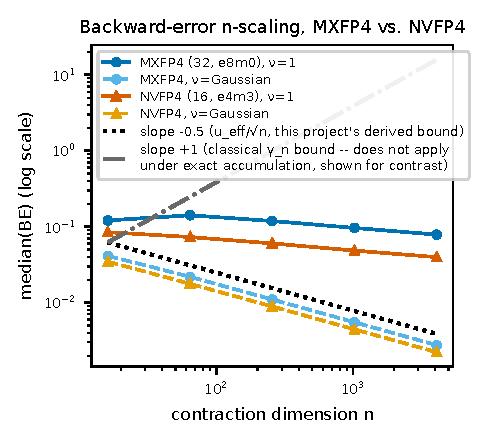
\includegraphics[width=\linewidth]{figures/figure2_n_scaling}
    \caption{Measured $\mathrm{median}(\mathrm{BE})$ against contraction length
      $n$ (log--log) for MXFP4 and NVFP4 at $\nu = 1$ and the Gaussian limit,
      against the obtained $u_{\mathrm{eff}}/\sqrt{n}$ slope $-0.5$ and the
      classical $\gamma_n$ slope $+1$ (shown for contrast, inapplicable under
      exact accumulation); the heavy tail decays far more slowly than $-0.5$.}
    \label{fig:n_scaling}
  \end{minipage}\hfill
  \begin{minipage}[t]{0.38\textwidth}
    \centering
    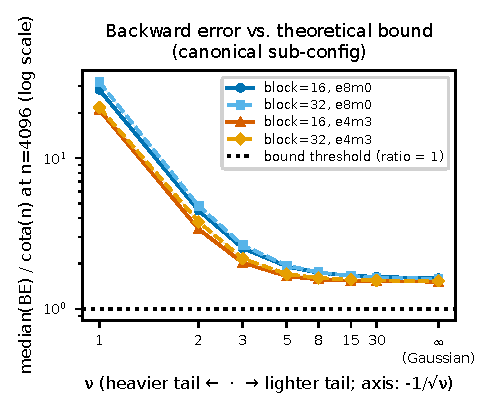
\includegraphics[width=\linewidth]{figures/figure1_nu_star}
    \addtocounter{figure}{1}% reserve Fig. 2 for the causal heatmap (Sec. 4.2)
    \caption{Median $\mathrm{BE}/\beta(n)$ at $n_{\mathrm{primary}} = 4096$
      versus tail index for all four block-size $\times$ scale-format arms;
      every curve sits above the ratio-$1$ threshold across the whole range, by
      roughly $20$--$32\times$ at $\nu = 1$ and $\sim$50--60\% at the Gaussian
      limit.}
    \label{fig:nu_star}
  \end{minipage}
\end{figure}

The empirical log--log slope of $\mathrm{median}(\mathrm{BE})$ against $n$ is
fitted by ordinary least squares for each of the 128 sub-configurations of the
sweep --- $8$ tail indices $\times$ $2$ block sizes $\times$ $2$ scale formats
$\times$ $2$ rounding modes $\times$ $2$ Hadamard settings --- over that
configuration's own 5 values of $n$, with a 95\% interval from 2000 bootstrap
replicates resampling each $n$'s trials independently. The reference is the
exponent $-0.5$ of (\ref{eq:bound}). Figure~\ref{fig:n_scaling} plots measured
$\mathrm{median}(\mathrm{BE})$ against $n$ for the two named presets; its
companion, Figure~\ref{fig:nu_star}, plots the same arms' error relative to the
bound $\beta(n)$ and is discussed in Section~\ref{sec:results:threshold}.

No configuration's interval contains $-0.5$; all 128 lie above it --- error
decays with $n$, but slower than the cancellation regime predicts, and nowhere
grows. That unanimity overstates the finding: it rests on a significance test
that at 1000--5000 trials excludes $-0.5$ even when the point estimate misses by
thousandths. By magnitude instead ($|\mathrm{slope} - (-0.5)| > 0.02$), 63 of 128
configurations deviate materially and 65 do not.

The split is ordered by tail weight, and the deviation shrinks smoothly and
monotonically as the tail lightens. At $\nu \in \{1, 2, 3\}$ every one of the 16
sub-configurations is material, with gaps from 0.041 to 0.490; the extreme is
$\nu = 1$, where the fitted slopes run from $-0.010$ to $-0.139$, one to two
orders of magnitude shallower than predicted rather than borderline. At
$\nu \in \{5, 8\}$ the sub-configurations straddle the threshold, some above and
some below, consistent with a smooth transition rather than a sharp cutoff. At
$\nu \in \{15, 30, \mathrm{Gaussian}\}$ none is material at any configuration, the
gap staying between 0.004 and 0.020.

The split follows the derivation's premises: the $-0.5$ exponent
(Section~\ref{sec:method:bound}) needs a mean-zero numerator behaving as a random
walk and a denominator obeying a law of large numbers --- moments the heaviest
tails lack ($\nu = 1$ is Cauchy). It is recovered to within 0.02 where those
moments exist and departs where they do not (Figure~\ref{fig:n_scaling}).

\subsection{Scale Format, Not Block Size, Is the Larger Lever}
\label{sec:results:decomposition}

The $2\times2$ design is read directly off the measured backward error, with no
theoretical bound involved. This partition is exploratory and post-hoc, adopted
under a dated preregistration amendment (Sec.\ 8.4) once the preregistered
$\nu^\star$ comparison (P1--P3) was left undefined by the finding of
Section~\ref{sec:results:threshold}. For each combination of tail
index, contraction dimension, rounding mode and Hadamard setting, three
statistics are formed in log space,
\[
\begin{array}{l}
  \mathrm{effect}_{\mathrm{block}} = \mathrm{median}(\log \mathrm{BE} \mid \mathrm{block}{=}16) - \mathrm{median}(\log \mathrm{BE} \mid \mathrm{block}{=}32) \\[3pt]
  \mathrm{effect}_{\mathrm{scale}} = \mathrm{median}(\log \mathrm{BE} \mid \mathrm{scale}{=}\mathrm{E4M3}) - \mathrm{median}(\log \mathrm{BE} \mid \mathrm{scale}{=}\mathrm{E8M0}) \\[3pt]
  \mathrm{interaction} = [\,(16,\mathrm{E4M3}) - (32,\mathrm{E4M3})\,] - [\,(16,\mathrm{E8M0}) - (32,\mathrm{E8M0})\,]
\end{array}
\]
each marginal effect aggregating over the other factor, with a 95\%
percentile-bootstrap interval from 2000 replicates resampling all four underlying
cells in one shared pass. Neither the tail index nor $n$ is collapsed.

Scale format moves the measured error more than block size does at every one of
the 40 canonical cells (8 $\nu$ $\times$ 5 $n$, round-to-nearest, no Hadamard
transform), and the ranking survives the secondary factors: scale format leads in
34 of 40 cells with the Hadamard transform on, 38 of 40 during stochastic
rounding, and 35 of 40 with both, never reversing to an overall block-size
majority in any of the four combinations. At $n = 4096$, canonically,
$\mathrm{effect}_{\mathrm{scale}}$ ranges from $-0.162$ at the Gaussian end to
$-0.389$ at $\nu = 2$, against $-0.042$ to $-0.246$ for
$\mathrm{effect}_{\mathrm{block}}$ (Figure~\ref{fig:causal_heatmap}): the
scale-format effect is about $3.9\times$ the block-size effect near the Gaussian
end, falling to roughly $2\times$ at $\nu = 2$ and about $1.1\times$ at
$\nu = 1$, where the two intervals still do not overlap (below). Both effects are negative at every
$n \ge 64$, so block $= 16$ and E4M3 --- NVFP4's two choices --- each reduce
measured error relative to their alternatives, and the larger of the two
reductions is the scale format.

The ranking is identical at all 5 values of $n$, at every $\nu$, with no crossing
anywhere in the grid, so the practical answer here --- unlike the threshold
analysis of Section~\ref{sec:results:threshold} --- does not depend on which $n$
had been designated primary. The $n = 16$ column is the apparent exception, and
it is not measuring block size at all: zero-padding leaves $\max|x|$ unchanged,
so a nominal block size of 32 spans the same 16 elements, with the same scale, as
block size 16 does. The effect first becomes measurable at $n = 64$, where the
two arms are genuinely different quantizers, and is essentially flat through
$n = 4096$ (at $\nu = 1$: $-0.286, -0.270, -0.257, -0.246$).

The margin $|\mathrm{effect}_{\mathrm{scale}}| - |\mathrm{effect}_{\mathrm{block}}|$
is thinnest at $\nu = 1$ (0.016 to 0.043 for $n \ge 64$) and wider on either side
--- 0.16 to 0.19 at $\nu = 2$, 0.124 to 0.135 at $\nu = 15$ --- but never
crosses: no point estimate flips at any of the 40 canonical cells, and at
$n = 4096$ the intervals are disjoint,
$|\mathrm{effect}_{\mathrm{block}}| \in [0.2395, 0.2510]$ against
$|\mathrm{effect}_{\mathrm{scale}}| \in [0.2719, 0.2831]$.

Backward error, not $u_{\mathrm{eff}}$, carries the headline comparison: it
determines GEMM output accuracy, whereas $u_{\mathrm{eff}}$
(Section~\ref{sec:method:bound}) is a per-element diagnostic. On $u_{\mathrm{eff}}$
the block-size effect leads at $\nu = 1$ and crosses the scale effect by
$\nu = 2$; in backward error the direction replicates but the crossing does not.
With the backward-error effects near parity for $\nu \le 2$, the clean ``scale
format dominates'' reading holds only at light-to-moderate tails, not the
heaviest ones that motivate the study.

The two factors are not purely additive: the interaction term is significant at
essentially every cell with $n \ge 64$, from $-0.095$ at $\nu = 1$ to $-0.028$ at
the Gaussian end at $n = 4096$. The dominance comparison above uses the pooled
marginal effects; at $\nu = 1$ the interaction is about a third of either main
effect, so that comparison is a simplification, not an exact partition.

\begin{figure}[t]
  \centering
  \addtocounter{figure}{-2}% reclaim the number reserved in the Sec. 4.1 two-up
  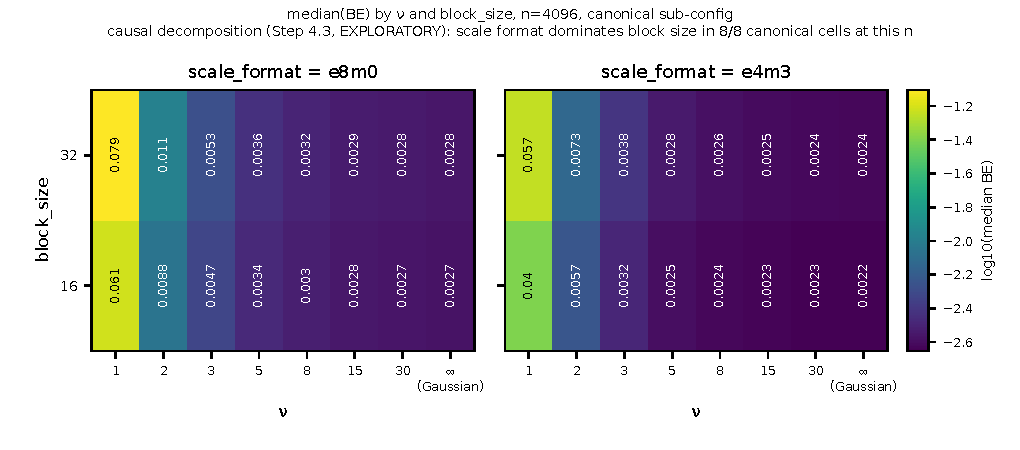
\includegraphics[width=0.66\textwidth]{figures/figure3_causal_heatmap}
  \caption{$\mathrm{median}(\mathrm{BE})$ over the block size $\times$ tail
    index grid at fixed $n = 4096$, split by scale format (E8M0 vs.\ E4M3);
    changing the scale format shifts the cells more than changing the block
    size at every $\nu$, though by a margin that narrows sharply toward the
    heaviest tail ($\nu = 1$).}
  \label{fig:causal_heatmap}
  \addtocounter{figure}{1}% restore counter past the two-up's Fig. 3
\end{figure}

\subsection{Why the Analysis Is Framed by Magnitude and Not by a Threshold}
\label{sec:results:threshold}

\looseness=-1 That decomposition replaced a preregistered plan: locate
$\nu^\star$, the tail index at which $\beta(n)$ first fails by the criterion of
Section~\ref{sec:method:bound}, for each of the 16 families, and compare the two
block sizes by where their $\nu^\star$ falls.

The bound is broken at every one of the 8 tested tail indices, in every one of
the 16 families, at $n_{\mathrm{primary}} = 4096$, and 0 of the 16 is
non-monotone, so $\nu^\star$ is not simply hard to locate but undefined
everywhere on this grid. For the two named presets, canonically, the median ratio
at $\nu = 1$ is 31.92 [31.85, 31.97] for MXFP4 and 20.91 [20.85, 20.97] for
NVFP4, against 1.588 [1.585, 1.590] and 1.515 [1.513, 1.517] at the Gaussian
limit. Even in the near-Gaussian regime, which the calculation's assumptions fit
best, the interval sits entirely above $1$: $c = 1$ under-predicts the measured
error by roughly 50 to 60\% there, and by a factor of 20 to 32 at $\nu = 1$
(Figure~\ref{fig:nu_star}).

This is not an artifact of the primary contraction dimension: the same pattern
holds at all 5 values of $n$, 16 of 16 families censored above and 0 below at
each. For MXFP4 at $\nu = 1$ the ratio is already 3.55 at $n = 16$ and rises
through 7.18, 12.10 and 19.62 to 31.92 at $n = 4096$, growing in line with the
shallower-than-$(-0.5)$ exponent of Section~\ref{sec:results:scaling} rather than
closing.

The preregistration anticipates this outcome: its all-cells-censored-above
contingency states the tail range was mis-specified, the hypothesis untestable on
such a grid, and the result to be reported as a grid mis-specification, not a
confirmation. It is equally not a null --- the rank comparison returns equal
fragility for the two block sizes only because every rank is pinned at the
ceiling, the signature of a saturated measurement. The two confirmatory results
therefore separate cleanly: the functional form of (\ref{eq:bound}) is well
supported at $\nu \ge 15$ (Section~\ref{sec:results:scaling}), while its leading
constant, fixed at $c = 1$ by the anti-circularity constraint of
Section~\ref{sec:method:bound}, is not calibrated anywhere in the tested range.

\looseness=-1 With no $\nu^\star$ to locate, block size and scale format could not
be compared through the bound at all --- both sides are censored past the edge of
what was measured. This is why Section~\ref{sec:results:decomposition} addresses
the same practical question directly from measured magnitudes, rather than
through the threshold criterion above.
